\documentclass{report}                                                           
        
\usepackage{titlesec}
\titleformat{\chapter}
  {\normalfont\LARGE\bfseries}{\thechapter}{1em}{}
\titlespacing*{\chapter}{0pt}{3.5ex plus 1ex minus .2ex}{2.3ex plus .2ex}
\usepackage[left=1in, right=1in, top=1in, bottom=1in]{geometry}
\usepackage{hyperref} 
\usepackage{xcolor} 
\usepackage{ulem}                     
\usepackage{graphicx} 
\usepackage{rotating}
                                                                                 
\newcommand{\note}[1]{\textcolor{blue}{\textit{note}: #1}}                       
\newcommand{\tristan}[1]{\textcolor{red}{TG: #1}}                                
\newcommand{\weird}[1]{\uwave{#1}}  


\begin{document} 
    \title{Pipeline systems and infrastructure for the efficient
            and open processing of Big neuroimaging Data} 
    \author{Valerie Hayot-Sasson}
    \maketitle 
    
    \begin{abstract}
         
    \end{abstract} 
    \tableofcontents
    \chapter{Introduction}
        In recent years, the volume of neuroimaging data acquired has exceeded
        both the storage and computation capacity of a standard research 
        lab workstation. With the advancement of data sharing technologies, 
        this data has been made widely available, however, accessibility to 
        such data remains limited due to infrastructural demands and lack of 
        performant software. Even with powerful infrastructure, such as High
        Performance Computing (HPC) infrastructure, software configured to 
        efficiently use resources is required to make execution time manageable
        . Ensuring efficient processing of data is 
        complex and limits accessibility to researchers with little programming 
        knowledge. Existing neuroimaging workflow engines primarily rely on HPC
        resource managers for performance and are therefore not well suited for
        BigData processing. As a result, frameworks for the efficient 
        processing of Big neuroimaging Data need to be developed\tristan{Add a sentence to transition from 'frameworks for efficient processing' to 'workflow engines'}
        
        Many neuroimaging workflow engines currently exist. Examples include
        Nipype~\cite{nipype}, Pipeline System for Octave and Matlab 
        (PSOM)~\cite{10.3389/fninf.2012.00007}, LONI~\cite{REX20031033}, 
        SPM~\cite{spm}, FastR~\cite{10.3389/fict.2016.00015},
        Automatic Analysis (AA)~\cite{10.3389/fninf.2014.00090} and 
        Pydpiper~\cite{10.3389/fninf.2014.00067}. These 
        workflow engines aim to satisfy four criteria: 1) simplified
        workflow composition, 2) performance, 3) portability of the workflows 
        and 4) reproducibility of the analyses. While these workflow engines
        do tackle performance, it is mainly limited to minimizing computation
        time and does not consider data transfer times -- which are typically
        costly in Big Data settings. Therefore, these engines need to be adapted
        for the processing of neuroimaging data.

        Big Data frameworks differ from those available in neuroimaging as their
        focus is mainly on workflow composition and performance. Big Data 
        frameworks such as Apache Spark~\cite{Zaharia:2016:ASU:3013530.2934664} 
        and Dask~\cite{rocklin2015dask} both aim to be easy-to-use,
        applicable to a wide variety of analyses and improve performance in the 
        processing of Big Data. These types of systems were primarily designed 
        to be efficient on commodity infrastructure in which transferring data
        over a network is extremely costly.

        Currently, there lacks a Big Data framework which is adapted for the
        processing of neuroimaging data. However, tools such as the Thunder 
        Project~\cite{Freeman:2014aa} allow for the processing of time-series
        neuroimaging data using Spark as the backend framework. Such tools
        provide built-in functions to process the data. For users to 
        extend functionality, it is necessary for them to understand the 
        backend framework. Other scientific workflow engines, such as 
        Toil~\cite{Vivian:2017aa} and Pegasus~\cite{DEELMAN201517}, have 
        incorporated features that enable more 
        performant workflow executions for scientific Big Data. They also enable
        the integration of Big Data frameworks as sub-pipelines within their 
        workflows. Despite integration with Big Data frameworks, it is not
        possible to create Big Data workflows using their API exclusively.

        A big limitation to adapting Big Data frameworks for neuroimaging 
        workflows is that these frameworks are tightly-coupled with the 
        infrastructure they were designed for -- commodity clusters. While
        it is possible for some research labs to be using either a local cluster
        or the cloud for their processing, many may only have access to HPC
        clusters. As a result of this, most available scientific workflow 
        frameworks have been designed for processing on HPC clusters. The 
        set-up of an HPC cluster is quite different from that of a commodity 
        cluster, and therefore, in order to effectively use Big Data frameworks
        for scientific computing, it is necessary to adapt the infrastructure 
        for processing on HPC.

        \tristan{Add a sentence to present the goal of the report.}
        This paper aims to evaluate the efficiency of current neuroimaging 
        frameworks in comparison to BigData frameworks and to determine the 
        extent to which BigData frameworks must be adapted to be effective
        neuroimaging workflow engines. 
        In section~\ref{datasets}, we will briefly introduce the two 
        types of datasets that are giving rise to the neuroimaging big 
        data. Section~\ref{platforms} will provide a brief introduction 
        to the data-sharing and processing platforms available to 
        researchers. We will conclude our 
        introduction on the differences between commodity and HPC infrastructure
        in section~\ref{infrastructure}.

        As we wish to evaluate and compare scientific workflow frameworks with
        Big Data frameworks for the processing of neuroimaging big data, we will
        break down our analyses by the four principal features necessary for
        effective neuroimaging workflow engines. The workflow engines discussed
        will include SPM, LONI, Nipype, PSOM, FastR, AA, Pydpiper 
        for neuroimaging; Taverna~\cite{doi:10.1093/bioinformatics/bth361}, 
        Pegasus, Make~\cite{10.3389/fninf.2016.00002}, 
        OpenMOLE~\cite{passerat2014openmole}, Nextflow~\cite{Di-Tommaso:2017aa}
        , Galaxy~\cite{Goecks2010}, 
        Toil for other scientific workflows; and Hadoop 
        MapReduce~\cite{Dean:2008:MSD:1327452.1327492}, Spark and Dask for
        Big Data Frameworks. Chapter \ref{workcomp} will evaluate these 
        workflows on the basis of workflow composition: we will % 'in other words' is on my list of expressions to avoid
        examine the programming languages necessary to construct these workflows
        , as well as, how easy is it to add new tools. In Chapter 
        \ref{performance}, we will proceed to 
        investigate the strategies employed by these frameworks to improve the 
        performance of their workflows. Chapter \ref{portability} will discuss
        the portability of the workflows written using these frameworks. 
        Workflow reproducibility will be then discussed in Chapter 
        \ref{reproducibility}.
        

        \section{Big Neuroimaging Datasets}\label{datasets}

            As a result of the rise in data sharing in neuroscience, 
            neuroimaging
            BigData has come to fruition. The field of neuroscience has now
            reached a bottleneck where there exists sufficient data to make
            impactful studies, but the software to process these datasets have 
            not evolved with the size of the data.

            Neuroimaging big data comes in two formats: 1) large images and 2) 
            large datasets. Large images consist of singular images ranging 
            from 100s of gigabytes to terabytes in size. A well-known example 
            of 
            such an image is the BigBrain~\cite{Amunts1472}, a histological 
            image 
            of the brain of a healthy 69 year-old man. At its highest resolution
            , it is 1x1x20$\mu$m or 1TB in
            size. Other examples of large images can be found in electron 
            microscopy (EM)~\cite{Hildebrand:2017aa}, polarized light imaging 
            (PLI)~\cite{10.1007/978-3-319-12084-3_1} and micro computational
            tomography (microCT)~\cite{10.1371/journal.pone.0035691}. 
            Images at 
            such high resolution are important to researchers as they provide 
            insights into aspects not otherwise detectible in images at lower 
            resolutions. However, due to their size and lack of resources 
            available to process such images, research on this data remains 
            limited.

            In contrast, large datasets consist of many images acquired from
            multiple subjects, which are too large to be processed in their
            entirety. Notable examples of these datasets include the 
            Alzheimer's Disease Neuroimaging Initiative 
            (ADNI)~\cite{doi:10.1002/jmri.21049}, 
            OpenfMRI~\cite{POLDRACK2017259}, 
            the Autism Brain Imaging Data Exchange 
            (ABIDE)~\cite{Di-Martino:2013aa}, the Consortium for
            Reliability and Reproducibility (CoRR)~\cite{Zuo:2014aa}, the Human 
            Connectome Project (HCP)~\cite{VANESSEN201362} and the UK 
            Biobank~\cite{Miller:2016aa}, with the later
            two being flagship recent examples of large datasets in 
            neuroimaging.

            The ADNI intiative is a collection of images (structural and 
            functional MRI, PET), urine,
            serum, cerebrospinal fluid biomarkers, as assessments (clinical and
            neuropsychometric) of 800 elderly subjects, which of whom 200 where
            healthy, 400 exhibited mild cognitive impairment and the remaining
            200 showed signs of Alzheimers. Imaging data is available both 
            pre- and post-processed form.

            OpenfMRI is a public repository originally conceived for the sharing
            of task-based fMRI data. Over time, it has grown to include EEG, MEG
            , resting-state fMRI (R-fMRI) and diffusion fMRI. Data made 
            available through
            OpenfMRI are obtained from both healthy and clinical individuals.
            Raw data must be made available for all datasets published to 
            OpenfMRI, however, preprocessed data may also accompany the raw data
            . At present, OpenfMRI houses data of a total 3372 subjects
            originating from 95 studies \note{obtained from website}.

            ABIDE was conceived to promote the advancement of knowledge 
            of Autism Spectrum Disorders (ASD). % inverted the sentence to keep symmetry with the other paragraphs
            ABIDE is an open repository of 
            preprocessed data obtained from 1112 R-fMRI datasets.
            In addition to R-fMRI, datasets also contain the corresponding 
            structural MRI and phenotypic data. As data made available in ABIDE
            is preprocessed, standardized pipelines were developed for the 
            preprocessing of the images. Popular neuroimaging processing tools
            such as CIVET~\cite{citation-0}, ANTs~\cite{avants2009advanced}, 
            and FreeSurfer~\cite{FISCHL2012774} were used for the 
            preprocessing of structural data, and several other pipelines were
            used for the processing of functional data.

            The Consortium for Reliability and Reproducibility 
            \tristan{expand acronym} was developed as an initiative to study 
            and improve the 
            reliability and reproducibility of functional connectomics. The 
            data made available by the Consortium consists of test-retest data 
            obtained from 33 datasets. The repository contains data from 1629 
            subjects, in which anatomical, R-fMRI, dMRI, CBF and ASL scans are 
            available \note{obtained from website}.


            The HCP initiative aimed to characterize the human connectome of 
            1200 healthy adults, ranging from 22 to 35 years of age, by studying
            twins and their non-twin siblings. Data collected for this initiave
            includes structural MRI, R-fMRI, task fMRI and dMRI. MRI data was
            collected using a 3T scanner for all participants, with a 200 
            participants additionally undergoing scans in a higher-resolution 7T
            scanner. MEG and EEG data is available for a subset of the subjects. 
            In addition to imaging data, behavioural and genetic data were also 
            acquired. To facilitate analysis for research groups, HCP made 
            available the raw data, minimally pre-processed data and processed 
            data. Pipelines were developed by the HCP for pre- and post-
            processing. As in ABIDE, these pipelines reused many commonly-used
            neuroimaging tools such as FreeSurfer and FSL for structural data
            and FSL and other tools for functional data. The total amount of
            data made available by the HCP reaches up to nearly 1 Petabyte.


            The UK Biobank is an initiative aimed at the detection of pre-
            symptomatic markers of diseases occurring in middle-aged to elderly 
            populations. The study will gather data from questionnaires, 
            physical and cognitive measures and biological samples of 500,000
            individuals. 100,000 of these individuals will additionally be 
            subjected to imaging studies. Imaging modalities used include
            structural MRI, fMRI and dMRI of the brain heart and body; low-dose
            X-ray bone and joint scans; and ultrasound of the carotid arteries.
            As with other initiatives, the UK Biobank makes available both 
            raw and processed data. This data is expected to exceed 0.2 
            Petabytes. Since processed data is provided, the UK Biobank makes 
            available it own pipelines based on tools in FSL, but also plans to
            adapt HCP pipelines from cortical surface extraction in their images
            .

            All these initiative stress the importance of data-sharing and
            large-scale studies for the advancement of science. Many researchers
            are limited to the processing of subsets of the data available as 
            they lack compute and storage resources to process the data in its
            entirety. It is also important to note that many of the pipelines 
            developed by these initiatives made use of popular neuroimaging 
            toolboxes, such as FSL~\cite{SMITH2004S208}, FreeSurfer, ANTS, 
            CIVET, rather than
            creating their own. Therefore, there is a great need for Big Data
            frameworks that can leverage existing tools for the efficient 
            processing of large-scale datasets. Widespread availability and 
            accessibility of such frameworks will in turn lead to a greater
            volume of higher-impact studies.


        \section{Open-science Platforms}\label{platforms}
            Efficient processing of workflows is only but a small portion of 
            the Big Data issue in neuroscience. % nice transition, this section gives more context for your study
            Sharing and storing of datasets
            and tools, secure access to and configuration of multiple computing 
            sites and provenance capture of all activities must be managed by 
            the researcher. This puts a heavy burden on researchers as they 
            require some knowledge of all these components in order to manage it
            correctly. These platforms also play a vital role in promoting 
            research through the sharing of knowledge. Users can choose to share
            their data and pipelines with others, reducing the need for others 
            to collect their own data or to develop their own workflows. It 
            also promotes robustness of results as the data and workflows will 
            be shared and tested by multiple users.

            Access to HPC resources may not always be straight-forward as 
            configuration must be adapted to the execution site. This can 
            range from scheduling policies, to available file systems, to 
            environment and available libraries. Platforms relieve the user
            from having to know site-specific details by providing seamless
            execution on any cluster the Platform has knowledge of.

            Examples of popular neuroinformatics open-science platforms include 
            CBRAIN~\cite{10.3389/fninf.2014.00054}, 
            OpenNeuro~\cite{gorgolewski2017openneuro} and 
            Neurodata~\cite{burns2018community}. OpenNeuro and NeuroData primarily focus on
            cloud deployement whereas CBRAIN is configured for the deployment
            of workflows on HPC resources. All three of these systems allow 
            users to configure, manage, share and execute their workflows with 
            the help of a web-based GUI. Integration with compute resources is
            entirely abstracted by the platforms. These platforms additionally
            provide tools to visualize their data.

            As neuroimaging workflow engines are typically best suited for 
            compute-intensive workflows, the workflows accessible in these 
            platforms are not expected to be as suitable to process the 
            volume of data made accessible by these platforms. Since these 
            platforms make various infrastructures available to researchers, 
            workflow engines must be adapted to efficiently execute on the 
            infrastructure made available.
            
        \section{Infrastructure}\label{infrastructure}
            HPC infrastructure was initially designed for the processing of 
            compute-intensive applications. As a result, \tristan{I disagree with 'As a result' and I don't particularly agree with the previous sentence: even if
            resources aren't scarce, they are good reasons to optimize resource managers: energy consumption, application makespan, fairness, etc. Also,
            I'm not sure if resources are less scarce now than they used to be: with the rise of computational sciences, almost every researcher now
            needs a cluster, and Compute Canada (but also other infrastructures) has been very busy.}
            resource managers for these systems employ
            strategies to efficiently use the compute resources available for 
            processing. However, with the advent of big data, data-intensive 
            workflows are now beginning to become more present on HPC systems.
            Since the schedulers and workflow engines made for HPC systems are 
            'data-unaware', they are not efficient with the processing of Big
            Data

            HPC and Big Data infrastructure differ in many ways. We define HPC 
            systems as those that employ a shared parallel 
            filesystem (distinct from any compute node), such as Lustre, and 
            data-unaware schedulers. \tristan{and data-unaware schedulers?}.
            \tristan{You should say that this definition is 'by contrast to big data platforms' to explain where it's coming from.}
            The shared parallel filesystem is the slowest of
            all storage devices found on HPC as it is shared amongst all users 
            of the system.
            Compute nodes in such infrastructure may not contain any local 
            storage. However, network interconnects between nodes are typically 
            fast.
            Resources managers used in HPC infrastructures typically employ 
            batch scheduling and execute heterogenous workflows. 
            Examples of schedulers used in HPC clusters 
            include SLURM~\cite{yoo2003slurm}, 
            PBS~\cite{10.1007/3-540-60153-8_34}, SGE~\cite{SGE} and 
            HTCondor~\cite{htcondor}.

            Big Data infrastructure \tristan{Call it 'Big Data infrastructure?'} differs from HPC infrastructures in that
            it uses less-costly hardware. It follows a shared-nothing paradigm
            where the storage is not shared between nodes. That is, all compute
            nodes are responsible for storing the data as well. File systems
            used within such infrastructure are distributed filesystems, such 
            as the
            Hadoop Distributed File System (HDFS)~\cite{5496972} and 
            Alluxio~\cite{Li:2014:TRM:2670979.2670985}.
            Fault-tolerance of the data is achieved through replication across
            nodes. As transferring data across the network is typically costly 
            in such infrastructures, frameworks designed to run on Big Data 
            infrastructure attempt to limit the transfer of data across nodes. 
            Resource managers created specifically for these systems
            typically expect dedicated infrastructure, as is the case with 
            Yet Another Resource Negotiator 
            (YARN)~\cite{Vavilapalli:2013:AHY:2523616.2523633}, but can also 
            execute heterogeneous workflows, as can be seen with 
            Mesos~\cite{hindman2011mesos}.

            Big Data infrastructure may also come in the form of cloud 
            infrastructure.
            While the hardware employed is typically the same as other
            Big Data clusters, the software used varies. Cloud infrastructures
            have the added benefit of virtualization, allowing users to 
            configure the infrastructure and software requirements to meet their
            needs. Cloud infrastructure also enables researchers to request
            dedicated resources without having to maintain these resources. One
            of the biggest limiting factors of cloud resources is the cost 
            associated with usage~\cite{10.3389/fninf.2017.00063}.

            Researchers typically have access to HPC infrastructure, but may
            also have access to Big Data infrastructure in the format of a 
            local cluster or cloud. Although both neuroimaging frameworks and
            Big Data frameworks can be configured to execute in either 
            environments,
            the performance enhancements that they bring are extremely
            dependent on infrastructure that they are executed on. For instance,
            neuroimaging workflows typically read and write to a shared file
            system at each workflow step. This is less of an issue in HPC 
            infrastructure as network bandwidth is typically better than on 
            commodity infrastructure. In contrasts, Big Data framework typically
            rely on there being some form of local storage. Employing a Big Data
            framework on HPC infrastructure may in turn result in less to no 
            data locality -- a strategy employed by Big Data frameworks to 
            minimize data movement across the network. Due to the variability in
            infrastructure available to researchers, a workflow framework good
            for neuroscience must be well adapted to handle these differences.

    \chapter{Workflow composition}\label{workcomp}

        Workflows, also known as pipelines, describe the flow of data from one 
        activity to another and are typically represented by a graph. \tristan{Not necessarily a DAG, see Nipype for instance, it has loops.
        I don't think you want to enter in a taxonomy of languages though, just say 'graph'}. Workflow activities, also referred to as 
        workflow interfaces or stages, encapsulate a tool through the use of an
        interface\tristan{Mention 'interface' here as an intro to sub-sec 2}. 
        Tools can be represented in many forms, including: command-line tools, 
        custom scripts integrated directly into the workflow code, web 
        services and software libraries.\tristan{A script is a command-line tool. I think tools may also be web services (Taverna) or just 
        software libraries (Dask)}. A workflow activity with all its 
        dependencies is considered ready to be staged.

        For a workflow engine to be considered successful, it must be simple to 
        compose workflows using that framework. New researchers should be able 
        to acquire the skills to compose worfklows without
        investing a significant amount of time in understanding it. Reuse of
        existing tools is also common occurrence in neuroinformatics, and 
        workflow engines need to accomodate this by undertaking a modular 
        approach and being easily extensible. With the sharing of data also 
        comes the sharing of workflows. For labs to share their workflows with
        the community at large, these workflows must be easily understood by the
        community. This relates to the reproducibility of studies, as it is 
        more than likely that easily understood workflows are reproducible. 
        \tristan{Perhaps mention that this also relates to the sharing
        of reproducible results -- VH: not sure if this is what you meant}.

        In this Chapter, we will compare and contrast the workflow composition 
        of seven neuroimaging frameworks (SPM, LONI, Nipype, PSOM, FastR, AA and
        Pydpiper), seven scientific workflow engines stemming from other fields
        (Taverna, Pegasus, Make, OpenMOLE, Nextflow, Galaxy, Toil), and three
        BigData frameworks (MapReduce, Spark, Dask). We will use two axes to
        evaluate workflow composition. Section~\ref{lang} will compare the 
        framework on the basis of programming language used. Section~\ref{ds}
        will then examine the differences in data structures between scientific
        and BigData frameworks. 
        Section~\ref{mod} will look at how easy it is to integrate existing 
        tools into the workflows.

        \section{Workflow language}\label{lang}
            The choice of workflow language (e.g. GUI, scripting language,
            programming language) greatly
            affects how easily it will get picked up by the community. Complex
            languages may mean greater efficiency of engines
            , but also result in extensive time spent on learning and developing
            the pipelines. Moreover, some researchers may not be well-versed in
            programming and may require very easy-to-use engines.

            To address this issue, some workflow engines have taken the role
            of employing a graphical user interface (GUI). This makes workflow 
            composition accessible to all researchers, including those with
            little to no programming background. The caveat to employing a 
            workflow engine with a GUI interface for workflow composition is
            that users are greatly limited by the tasks they can perform. For 
            instance, workflows that perform any form of iterative operations
            (e.g. machine-learning workflows) or workflows with conditionals
            (e.g. given a certain input, do not execute this activity) cannot
            be represented by a GUI. 
            Workflow engines that employ a worfklow composition GUI include:
            SPM, Taverna, OpenMOLE, LONI and Galaxy.
            \tristan{My conclusion on GUIs is that they are suitable only
            for very simple pipelines. Perhaps the intro could give an idea
            of the types of pipelines encountered, showing a simple one and
            a more complex one. No way fmriprep is described in a GUI.}

            As more experienced programmers may feel limited by a GUI, workflow
            engines have decided to provide users with the ability to describe
            their workflows in more flexible formats. Even those with GUIs for 
            workflow composition, such as LONI and OpenMOLE, allow more 
            experienced users to script their workflow. Four different 
            languages are used for describing scientific workflows: 1) Python, 
            2) MATLAB and GNU/Octave \tristan{I think the official name is GNU/Octave}, 3) Shell Scripting languages \tristan{scripting languages}, 4) Domain Specific Language (DSL). \tristan{I don't see why CWL and XML don't qualify as DSL} Workflows engines that 
            employ usage of Python include: Nipype, FastR, Pydpiper, Pegasus, Toil,
            MapReduce, Dask and Spark. \tristan{Dask? Spark?}.
            Python is an excellent choice as a programming language for 
            scientific workflows, particularly neuroinformatics, due to its 
            widespread use within the community. Other advantages of 
            programming in Python include: a wide array of available libraries,
            particularly neuroimaging-specific ones such as Nilearn~\cite{nilearn} and Nibabel~\cite{matthew_brett_2018_1287921}
            and more general, but heavily used in neuroimaging, libraries such
            as SciPy~\cite{scipy} and Scikit Learn~\cite{pedregosa2011scikit} \tristan{mention scipy, sci-kit learn, etc}
            , and an lower learning curve compared to other 
            programming languages. Additionally, Python is platform independent
            meaning it can be installed on any system. In terms of BigData 
            frameworks that employ Python, Dask is exclusively written in Python
            , whereas Hadoop MapReduce and Spark both have interfaces to Python
            while being written in Java and Scala, respectively.

            Another widely-used high-level programming language in the 
            neuroinformatics community is MATLAB/Octave. Workflow engines which
            use this language include: PSOM, SPM, and Automatic analysis. Like 
            Python, MATLAB and GNU/Octave are platform-independent and also easy to use. In addition, MATLAB has 
            been found to exhibit better performance compared to Python for 
            common technical tasks. It also provides an integrated environment
            for programming. A 
            downfall to imposing MATLAB as programming language is that it is proprietary, thus imposing a fee on 
            anyone wishes to program in that language or have access to their diverse array of libraries \tristan{You should also mention the
            advantage of Matlab: easy to learn, integrated ecosystem, 
            performance, see 
            \url{https://www.mathworks.com/products/matlab/matlab-vs-python.html}}. 
            To offset this, PSOM ensure compatibility with the GNU 
            Octave programming language, thus 
            removing the requirement to purchase software for workflow 
            composition. 

            \tristan{This paragraph should start with ``Shell scripting ...". The structuration of this section by language
            is great, but the writing of this paragram doesn't put it forward.}
            Many researchers have been exposed to Shell scripting languages as 
            several scientific workflows are composed in UNIX-based 
            environments. These environments typically have Make installed by
            default eliminating the need for users to install it manually.
            These features make workflow engine Make desirable for scientific
            computing.
            As Make is exclusive to UNIX environments, it is not 
            platform-independent. However, Make has the flexibility of being
            easily extensible and can interface directly with any command-line
            tool. Shell scripting, nevertheless, is generally not as intuitive
            as programming languages like Python and MATLAB.

            Domain Specific Languages (DSL) are also used to compose workflows.
            The can be made up of any language (e.g. XML, CWL, Scala and Groovy) that has been adapted for use in 
            a specific domain.
            XML is the language of choice in  
            workflow engines such as Pegasus and LONI. Using a markup language
            such as XML have the advantage of having access to 
            language-independent parsers and validators. However, the use of a 
            markup language removes some of the flexibility. \tristan{Before you explain the downside, 
            you should say what are the advantages: mainly language-independent parsers and validation.} Users wanting to 
            include 
            custom scripts as workflow activities must do so by creating a 
            command-line interface for their custom script. Pegasus, however,
            does provide many interfaces to describe the pipeline in including
            Java, Python and Perl.

            Another example of a DSL is a Common Workflow
            Language (CWL). CWL can be seen in workflow engines like Toil. 
            It is similar to XML in that its main difference is that it is 
            YAML/JSON-based.
            \tristan{It is a YAML-based DSL for workflows. Just like Pegasus' DAX is an XML-based DSL}. Files can either be written in JSON or YAML formats. CWL is 
            based on workflow engines like Make \tristan{? I don't think CWL relies on make, does it?}, but differs in that tasks
            are isolated \tristan{inputs and outputs are somewhat explicit in a Makefile}. Similarly to 
            make, CWL is only available on Linux and OSX platforms \tristan{strange, the CWL interpreter is in Python so I'd expect it to run anywhere}. \note{cite cwl 
            website}

            Programming language-based DSL workflow engines include OpenMOLE, which is  
            derived from Scala, and Nextflow \tristan{Nextflow?}, which is derived from the Apache 
            Groovy programming language. While both are written on top of the 
            Java platform, Nextflow is only compatible with Linux and OSX \tristan{How about using Linux everywhere instead of UNIX-based?} 
            environments. These programming languages are not otherwise commonly
            used in neuroimaging, meaning that users must learn specific 
            languages that would not otherwise be used in their field.

            With the exeption of LONI, neuroimaging workflows tend to stick to
            commonly used programming languages such as Python and MATLAB/Octave
            . This is likely due to the fact that the learning curve to adapt to
            these languages is relatively low and users can harness the 
            flexibility of these languages. 
            
            Since MapReduce, Spark and Dask all provide interfaces to Python,  
            they are good candidates for neuroimaging workflow engines. In addition
            Spark also interfaces with R, another programming language commonly
            used in neuroimaging.

            \section{Data structures}\label{ds}
                
                The data structures made available by workflow engines dictate
                the maximum performance available to a workflow. Scientific
                workflows are generally file-based, meaning that data, in the 
                form of files, will be 
                transferred across the network and I/O must be
                performed at each workflow activity. It is possible for some 
                data to remain in memory with scientific workflows, but these 
                are typically basic types such as numbers, strings and lists.
                More complex types, however, can be seen in workflow engines 
                such as PSOM which accept nested structures as long as the
                structures's terminal fields are either strings or cells of 
                strings. Due to workflow engines being file-based, performance
                is limited, particularly with BigData.
                
                In order to improve performance, BigData frameworks introduced
                data-centric data structures. MapReduce is key-value based, 
                therefore, data with the same keys would be located at the
                same nodes. As MapReduce still requires file-based I/O, the 
                amount of I/O remains similar to that of scientific workflows. 
                However, the key-value structures help to reduce the amount 
                of data transfers by promoting data-locality.

                The MapReduce key-value pair data structure is an effective 
                data structure for describing workflows, but is limited to only
                batch workflows and can be improved in terms of performance. 
                The resilient distributed datasets 
                (RDD)~\cite{Zaharia:2012:RDD:2228298.2228301}, Spark's main
                abstractions addresses these 
                issues by being a shared-memory structure. They 
                are immutable and only permit coarse-grained edits to ensure 
                fault-tolerance. The RDDs shared memory enables a reduction in
                I/O operation as data can be maintained in memory. Spark will only read 
                and write data to and from disk when data exceeds available 
                memory or when data needs to be shuffled around, as is the case
                with all Spark actions and certain transformations such as 
                \textit{join} and \textit{reduceByKey}. Moreover, RDDs permit
                workflows to be evaluated lazily. By being able to look at the
                entire workflow before evaluation, Spark can select the most
                performant methods for evaluating the data. 
                The RDD additionally expands its use to additional applications
                by enabling the expression of both iterative and interactive
                workflows. Furthermore, Spark provides an additional data 
                structure to enable the efficient processing of tabular data.
                This data structure is know as the 
                DataFrame~\cite{Armbrust:2015:SSR:2723372.2742797}.

                Dask builds off of Spark by not only providing data 
                structures similar to Spark's RDDs and Dataframes, Dask Bag and 
                DataFrame, but by also providing an abstraction for 
                larger-than-memory matrices, the Dask array. Furthermore, it is
                possible to use common Python APIs (e.g. NumPy\note{cite} and 
                Pandas DataFrame~\cite{mckinney2011pandas}) to process the 
                data. Although Spark does not have a datastructure for large 
                matrices, it has an RDD-based API, known as \textit{linealg}
                for similar processing of large 
                matrices~\cite{BosaghZadeh:2016:MCO:2939672.2939675}.

                
            \tristan{So this is now about data structures, not just language.
            This is really excellent, but this should perhaps go into a 
            specific sub-section. I think you could mention that 
            scientific workflow engines traditionally rely on files 
            only, and simple types, but that big data engines have 
            invested a lot in data structures, starting from key-value 
            pair representations in MR to RDD and Dask arrays. Spark is 
            actually built around RDDs, this is salient-enough to be 
            discussed a bit more. It actually makes a lot of sense that 
            data-focused engines are built around data structures 
            instead of control constructs. The ACM Com Spark paper makes it clear
            that unifying data structures is key to performance and interoperability, 
            because it allows data to remain in-memory instead of having to go back
            and forth to different environments. I would only mention linealg 
            in the description of Dask arrays. So, how about a 
            sub-section 'data structures' with 4 paragraphs: (1) 
            scientific and neuroimaging engines, (2) Big-Data, MR, (3) 
            Spark's RDDs and DataFrames, (4) Dask arrays, mentioning 
            linealg. } 


        \section{Tool interfaces}\label{mod}
            \tristan{Since this section is about interfaces, I would
            rather call it ``Interfaces" or ``Tool interfaces".}
            Often times, users will want to integrate existing tools into their 
            workflows. In order for workflows to communicate effectively with
            the tools, it is required that an interface be created. Workflow 
            interfaces may range from simple command-line calls, to more 
            complex interfaces that track inputs, outputs and other parameters. 
            Furthermore, they ensure
            that all necessary parameters are correctly defined and in the 
            correct order,  capture all of the 
            standard input/output and create folders to encapsulate task inputs
            and outputs. Early scientific workflow engines, such as SPM, are 
            monolithic. As a consequence, these workflow engines do not provide
            a complex class for interface definition and validation. Recent
            Workflow engines take a modular approach and promote sharing of data
            and pipelines. Thetypically rely on more complex types 
            of interfaces in order to ensure correct functioning of the pipeline
            . Since these interfaces can be rather complex, it is necessary for the 
            workflow engine to provide an intuitive way for users to create 
            interfaces for their custom tools. Workflow interfaces can be 
            divided into two groups: those that are described using a 
            programming language and those that are described using DSL.

            Making the choice between a programming or a markup language for 
            interface definition is not obvious. One of the main reasons for 
            selecting a programming language is that programming language is 
            more versatile than are markup language, allowing any type of 
            operation to be defined. For instance, a dynamic number of outputs
            can be generated using a programming-language based interface 
            definition. Workflow engines that utilize programming 
            languages for the 
            description of their workflow interfaces include: Nipype, PSOM
            , Pydpiper, Toil, OpenMOLE and Make interfaces. 
          
            Nipype's wrapper, written in Python, can encapsulate CLIs, SPM, 
            MATLAB and Python scripts. InputSpec and OutputSpec are two classes 
            that can are used to describe the inputs and outputs of the 
            interface. The former defines the input parameters of 
            a command and the latter defines the outputs that are possibly 
            generated by the command. For CLIs, it is necessary to describe the
            command, such as order of parameters and required and optional parameters. 
            Apart from Input and Output Spec, a Python dictionary containing all
            expected outputs can be included.
            Before executing a CLI, Nipype can start X virtual framebuffer if 
            user interaction through a GUI is required by the tool if specified. 
            For SPM interfaces, the job 
            type and name must be specified. Interfaces to MATLAB require 
            definition of the run function, while Python interfaces require
            the definition of the \textit{\_run\_interface} function. \note{from
            website}.
            
            PSOM’s tool interfaces are known as \textit{Bricks}. They are a 
            little less versatile than Nipype'sinterfaces since they can only
            interface with MATLAB functions or CLIs. Bricks require the 
            definition of input and output files, in addition to a structure of 
            program options. A useful feature found in PSOM is the ability to 
            perform a “dry-run” of the Brick without executing the command.

            Pydpiper's tools can either be custom Python code or CLIs. The 
            \textit{PipelineStage} and \textit{CmdStage} are used to 
            encapsulate the tools. The \textit{CmdStage} class is specifically 
            used to interface with CLIs, and thus, accepts a parsed array of the
            command and its parameters as input. Atoms, typically used to wrap
            around MINC file-format related tools, inherit from the
            \textit{CmdStage} class, and require the input MINC file (string or
            file handler) to be provided. A output file can also be specified, 
            but it must be of the same format as the MINC file (string or file 
            handler). Additionally, it is possible to pass multiple optional 
            arguments to the Atom.

            Toil is another workflow engine that describes their tool interfaces
            in Python. The wrappers, also known as \textit{Jobs} enable users to
            interface with custom Python code or Dockerized \cite{merkel2014docker} 
            CLIs. Interfaces can be constructed either by creating a class that
            inherits from the \textit{Job} class or through the use of a 
            built-in function that converts the user-defined function (UDF) to a 
            Toil \textit{Job}. To convert, all that is required is the UDF,
            however, the user may also choose to include details on memory, 
            number of cores and disk space required. For Dockerized tools, Toil
            provides a built-in function that accepts the tool name, working dir
            and parameters of the tool.

            OpenMOLE has the ability to encapsulate UDF Scala scripts and CLI. 
            In the case of CLI tasks, it is also possible to containerize or 
            encapsulate with CARE \note{cite} to make it portable. OpenMOLE
            defines several classes to allow for the execution of different 
            types of tools. Like other framworks, it is vital to describe the
            inputs and outputs of the Tasks such that the execution of tasks 
            can be performed. 

            The Make pipeline is expressed in a makefile containing a set of 
            rules (Tool interfaces). Rules consist of three components: targets, 
            dependencies and recipes. The target is the output (typically a 
            file) of the 
            execution of a recipe and the dependencies are the input required to 
            produce the given target. Recipes are the shell commands that will
            generate the target from its dependencies. 

            \tristan{Users can still integrate tools as Matlab functions
            doing system calls}.
            Although DSL-based workflow interface schemas may be less versatile
            than those written using programming languages, DSL based schemas
            can be reused by any engine. This allows interface schemas to be 
            portable. AA, LONI, FastR, Taverna, Pegasus and Galaxy all 
            implement their iterface definition using a DSL.

            AA 
            allows users to define their tasks through XML specification. AA's 
            XML tasklist is simply an ordered list of tasks which also includes
            details on analysis-specific parameters. Dependencies are
            inferred by the program through analysis of the module interfaces.
            Module interfaces consist of MATLAB user script and an XML 
            descriptor. The descriptor contains details on the input and output
            data stream types (e.g. epi, structural, dicom\_header) 
            and the desired domain (e.g. study, subject, session). During 
            execution, each task is given its own unique folder to operate on. 
            The engine will copy data to and extract data from this folder.

            LONI enables generation of 
            the XML-based module interface through its GUI. The module interface
            consists of details on \note{from website} module metadata (e.g.
            authors, package, version, name) and citation information, 
            command-line syntax, parameter and file types, dependencies and 
            output and error handling.

            FastR allows for the definition of workflow modules in both XML and 
            JSON. Module definitions are broken down into two components, 
            \textit{Tool} and \textit{Interface} class. The \textit{Tool} is the
            component that is written in either XML or JSON. It defines three
            components: general metadata, target and interface. General metadata
            consists of details such as name, version and authors. The target, 
            on the other hand, consists of details on the execution environment
            (e.g. operating system, interpreter and binary file). The last 
            component of the \textit{Tool}, the interpreter, provides details on
            the inputs and outputs of the tool (e.g. name, datatype, cardinality
            , location). FastR provides to schemas to validate and convert the 
            \textit{Tool} to a Python object
            : the \textit{Tool} schema and \textit{FastRInterface}. Should these
            schemas not meet the requirements of the user, the user may choose 
            to define their own schema.

            Tool addition in Taverna is primarily performed through the user 
            interface, but can also achieved through the creation of an XML
            descriptor. Taverna differs from other workflow engines in that it
            can 
            execute generic-style services (i.e. WSDL and REST) in addition to
            other types of Web Services, external CLIs, R scripts and
            Java services. To interface with a CLI, the XML file must contain 
            the command to execute, file inputs and outputs (if required), if 
            standard input, output and error streams must be conserved and the 
            location where the command should execute\note{from website}.

            Pegasus is another workflow engine that uses an XML format to 
            define the CLI tools interface. The XML interfaces are typically 
            incorporated directly into the workflow DAX definition. However, a 
            separate multiline text-based 'Transformation Catalogue' file can
            be provided. Information encoded within the interfaces include
            tool identifier (typically namespace::version), the URL or filepath
            to the executable, site identifier of the executable's host, 
            executable type (e.g. installed or staged) and the profile. In
            addition to UDFs and CLIs, Pegasus
            can also execute containerized tools \tristan{how about the other ones?}. For this, a container 
            identifier, image URL, site identifier of the image, and container
            profiles must also be defined \note{from website}.

            While Galaxy is primarily a GUI-based application, an XML tool
            configuration file is required to add the tool to the application.
            The tool wrappers\ schema is very rich allowing for many tool 
            features to be defined. Similarly to many other workflow engine tool
            wrappers, the configuration file contains details on the tool name, 
            type, id, versions, command and input and output specifications. It
            also enables the execution of containerized tools. Furthermore,
            Galaxy enables users to specific actions to be performed on the 
            output files once created and define test cases.

            Unlike scientific workflow engines, BigData frameworks do not 
            provide default interfaces for the execution of complex tools 
            written in 
            languages different from their own. While Dask users can reference
            UDF Python functions directly in their workflow, Spark users
            must define a lambda function within an action or transformation 
            that executes their UDF or library on the data. Similarly to Spark,
            functions referenced in MapReduce must be called from within a Map
            or Reduce task. MapReduce can additionally reference Java 
            code and Spark can call on code also written in Scala, Java and R.

            For all workflow engines that do not, by default, interface with 
            command-line tools or containers, there are libraries that can be
            easily integrated to achieve that. 
            Boutiques~\cite{doi:10.1093/gigascience/giy016}, for instance, is a 
            Python library that can execute command-line or containerized tools
            defined within a JSON schema. Furthermore, the library's richness
            compete with Galaxy's XML. Python-based BigData frameworks can 
            easily call on this library from within the workflow in order to
            communicate with the tools.

            \tristan{Good material in here, but it lacks a bit structure.
            I like your structure of the previous sub-section, by language. I think
            here you could have two groups: (1) DSL descriptions (XML, JSON, etc) and (2)
            Python or Matlab descriptions. One advantage of DSLs is that they can 
            be more easily reused in different engines, while programming languages
            are more flexible, for instance Nipype allows outputs to be specified
            at runtime (dynamic number of inputs with names only known after
            the interface ran.)}


            
    \chapter{Performance}\label{performance}
        Neuroimaging frameworks are notoriously known to be compute-intensive.
        The workflows and their respective tools needed to incorporate 
        parallelism in order to save on computing time. Maintaining good 
        performance has become especially critical now that neuroimaging
        BigData has emerged. The dichotomy remains between scientific 
        workflows and BigData workflows. While scientific workflows have made
        advances towards more performant engines, they still lack the 
        strategies BigData frameworks employ to reduce data transfers. 
        
        Another notable aspect to consider is that both types of engines 
        (scientific and BigData) are tightly coupled to the infrastructure
        they were intended to be used on. Scientific workflow engines
        try to remain efficient in their handling of compute resources since such
        resources were previously scarce. In contrast, BigData frameworks 
        make efficient use of commodity clusters, where data transfers are 
        burdensome, particularly when faced with BigData.

        As some researchers are trying to shift towards the use of commodity 
        infrastructure while others are trying to process BigData on HPC, the 
        ideal workflow engine must run efficiently regardless of 
        infrastructure available. Otherwise, researchers are either left with
        workflows running inefficiently on resources or having to learn 
        multiple frameworks and rewrite their workflows depending on the 
        infrastructure selected.
 
        In this Chapter, we will compare scientific
        workflows to BigData frameworks on the basis of performance. 
        Section~\ref{fs} will look at what filesystems are supported \tristan{supported?} by the 
        engines. This is important because data movement of any kind is costly,
        and may be worse depending on the filesystems available. Furthermore, 
        typical neuroinformatics pipelines manipulate files, and therefore, 
        reducing the amount of I/O is necessary.\tristan{Also, mention that neuroinformatics
        pipelines manipulate files.}
        Section~\ref{sched} will provide an overview of the schedulers 
        available and their compatibility with the workflow engines. 
        Section~\ref{other} will discuss the checkpointing of data in the context
        of scientific workflows. This chapter will conclude with a discussion
        on the efficacy of Big Data frameworks for scientific computing, in
        Section~\ref{eval}.
        
 
        \section{Data-centric optimizations}\label{fs}
            
            
            Although MapReduce, Spark and Dask are all data-intensive worflows,
            Dask can be more similar to that of scientific workflow, 
            particularly in a multiprocessing environment. It focused on the 
            efficient 
            scheduling of tasks and relies on I/O and network transfers to
            communicate the data between nodes. With BigData workflows, such
            operations could incur significant performance penalties. 
            To mitigate this issue and remain efficient in the face of
            BigData, Spark and Dask implement data locality, lazy evaluation 
            and in-memory processing. Data locality is the scheduler's ability
            to schedule tasks nearest to data location to reduce data transfers.
            Lazy evaluation is the workflow's ability to optimize performance
            based on the pipeline's graph structure. In-memory processing, on 
            the other hand, tries to remove any I/O that occurs between tasks. 
            Platforms such as MapReduce rely heavily 
            on I/O, but the 
            I/O performed occurs on the compute node rather than on 
            shared storaged, making it generally more efficient than scientific
            workflows. Additionally, MapReduce uses the concept of 
            locality to ensure limit data transfers across the network.
            For the efficient processing of neuroimaging BigData, it will be
            necessary for scientific worflow engines to incorporate these 
            strategies.
        

            \subsection{Strategies}
                \subsubsection{In-memory computing}
                    Random Access Memory (RAM) is the fastest memory available
                    to workflow engines. BigData frameworks, such as Spark and 
                    Dask, leverage this feature by maintaining data in memory 
                    between tasks rather that saving them to local disk or 
                    shared memory which may incur significant overhead.

                    Spark and Dask can both read from filesystems available to
                    all nodes. When an action (Spark) or a compute (Dask) is 
                    called, the data is read from the storage and uploaded into
                    memory. Tasks use the data located in memory to compute the
                    results. Should data not fit in memory, the results may 
                    spill to local disk, if local storage is available. 
                    Otherwise, the engines will spill data to a shared 
                    filesystem. The later is a common case in HPC systems as 
                    storage and compute resources are typically separate, 
                    however, these shared filesystems are typically slower than 
                    local storage, and therefore, there will be additional 
                    performance penalties.

                    As data is not stored within a resilient distributed 
                    filesystem such as Lustre and HDFS, it risks being 
                    permanently lost if a node failure occurs. Spark and Dask
                    have both addressed this through the notion of 
                    \textit{lineage}. Lineage refers to the set of operations
                    that the data has undergone. By recording the lineage, lost
                    data will always be recoverable as the set of operations
                    to reproduce the data are known. Should a node be lost to 
                    the cluster, Spark and Dask reschedule the tasks required 
                    to rebuild the dataset to other nodes.

                    As subsets of the lineage can be reused amongst different
                    structures in the pipeline, it is possible to cache the 
                    data in order to avoid any form of recomputation, which 
                    could otherwise incur performance penalties.
                                      
 
                \subsubsection{Data locality}
                    Data locality, with respect to BigData frameworks, is a
                    scheduling
                    strategy in which location of the data is known by the 
                    scheduler and tasks are scheduled to the location where the
                    necessary data is located. It was one of the first main 
                    strategies implemented to make BigData processing more 
                    efficient. The reasoning behind data locality is that 
                    network transfers are expensive, particularly within 
                    Big Data infrastracture, and therefore transferring large 
                    volumes of data across the network for every task would be 
                    rather expensive.

                    While MapReduce and Spark both partition data across the 
                    network similarly, they achieve data locality slightly 
                    differently. MapReduce can use the local filesystem in 
                    standalone mode, but requires use of a distributed 
                    filesystem executing on the compute nodes such as the 
                    Hadoop Distributed File System (HDFS). The reason as to why
                    parallel file systems such as Lustre do not work is that 
                    the storage nodes on such file systems are separate from 
                    the compute nodes. Separate storage and compute nodes 
                    eliminate any possiblity of data locality as network 
                    transfers will occur regardless of storage node. When the 
                    next MapReduce task is available, the master node will 
                    query the distributed file system to determine the 
                    available nodes closest. The master will first attempt to
                    schedule the task on a node containing the data, but if 
                    that node is not available, it will attempt to schedule
                    the task on the same rack. If all else fails, the task will
                    be scheduled on a node found on a different rack. 

                    In contrast to MapReduce, Spark and Dask do not require 
                    data to 
                    be stored on a HDFS-like filesystem. They can read data 
                    from
                    any form of shared-filesystem, including Lustre. If data 
                    is extracted from a non HDFS-like filesystem, the initial 
                    loading of data will not use data locality. However, in all
                    future tasks in which the data is already loaded into an 
                    RDD, the scheduler will be able to assign task to the most
                    favorable partition dictated by delay scheduling according
                    to data locality.

                    
                \subsubsection{Lazy evaluation}

                    Lazy evaluation is a strategy used throughout computer 
                    science to improve performance of operations. Rather than
                    evaluating a expression immediately, it will wait until it 
                    is required in order to compute the result. This is 
                    achieved in Spark through the calling of an \textit{action}
                    on an RDD and in Dask through the calling of a 
                    \textit{compute} function on one of its data structures.
                    By using lazy evaluation, the engines are capable of 
                    constructing graphs that result in the most optimal
                    task order of execution and further save on data transfers. 
                    \tristan{And further save on data transfers}

            \subsection{BigData Filesystem optimizations for HPC}

                Writting BigData to Lustre is very costly compared to local 
                node storage. Distributed filesystems found on HPC 
                infrastructure provide their own form of fault-tolerance, 
                therefore, adding a BigData filesystem such as HDFS which 
                replicates the data may burden the storage layer only to 
                providea feature which already exist. This is especially 
                problematic as storage on HPC compute nodes may be limited.
                Moreover, while BigData frameworks typically execute on a 
                dedicated BigData cluster, they will be on a shared cluster in
                HPC, with many processed trying to access the memory. The 
                following are two optimizations made for the storing of BigData
                .

                Alluxio~\cite{Li:2014:TRM:2670979.2670985}, 
                formerly known as Tachyon, is an in-memory filesystem
                that stores lineage data to offset the cost of writing data to 
                disk. The assumption that Alluxio makes is that it will be less
                costly to recompute the data that to store the data to disk and
                replicate across the network for fault tolerance. However,
                unlike Spark applications, Alluxio is meant to run indefinitely
                , making it unfavourable in some cases, to recompute the data
                from its starting point. For this, Alluxio evaluates the 
                lineage data and checkpoints the files which have been 
                repeatedly accessed (i.e. hot files). This strategy also helps 
                in avoiding the checkpointing of intermediary files. 

                Triple-H~\cite{7152476} leverages the heterogeneity of HPC 
                clusters to 
                optimize the data's placement across the cluster for most 
                efficient use. It aims to reduce the I/O bottleneck of writing 
                through data buffering and caching. Triple-H has two modes of
                operation, Default and Lustre integrated,
                that allows it to execute on systems both with and without 
                access to a distributed filesystem. To further reduce I/O in
                HPC systems, Triple-H leverage's Lustre's fault tolerance 
                instead of using HDFS's replication-based fault-tolerance. 
                Triple-H improves 
                performance of cluster I/O by writing the data to
                the most optimal storage layer (RAMDisk, SSD, HDD, Lustre) 
                dictacted by the selected placement policy (i.e. Greedy or 
                Load-balanced). This allows alternative storage to be used as 
                a form of burst buffer to Lustre as data is written into a more
                optimal storage layer before being transferred to a slower 
                storage such as Lustre. 

                Although both of these solutions have shown to improve I/O
                performance, their benefits are limited to certain 
                configurations. Alluxio needs to be installed throughout the 
                cluster occupying available memory. Data locality may also be
                and issue as the user may only be scheduled to a subset of
                nodes that do not store the data. Moreover, neuroimaging 
                operations are compute-intensive, with some tasks being 
                extremely lengthy. Recomputation may not be affordable and long
                tasks can be frequent, meaning Alluxio will need to store more 
                data that desirable.

                Triple-H's main limitation is that it assumes the compute nodes
                have local storage. This is certainly not always the case and
                any performance improvements in systems without local storage 
                may be negligable at best.   
            
        \section{BigData Scheduling}\label{sched}
            
            Scientific workflows typically rely on HPC schedulers for 
            distributed scheduling on clusters. These schedulers include 
            SLURM~\cite{yoo2003slurm},
            PBS~\cite{10.1007/3-540-60153-8_34}, 
            TORQUE~\cite{computing2015torque}, 
            SGE~\cite{SGE}, HTCondor~\cite{htcondor} and 
            Mesos~\cite{hindman2011mesos}. Additionally, they may provide
            their own form of scheduling for computations on a single node. 
            BigData frameworks, such as Dask,
            also provide interfaces to these HPC schedulers. However, other
            frameworks such as MapReduce and Spark are limited to Big Data 
            schedulers such as Yet Another Resource Negotiator (YARN) and MESOS.
            The reason MapReduce and Spark do not leverage HPC resource managers
            is that HPC resources managers are unaware of the locality of the 
            data and cannot perform any form of lazy evaluation.
            In addition to YARN and MEsos, Spark provides its own standalone 
            scheduler. The standalone scheduler is simple providing only a 
            basic scheduler. It allows users to use Spark out-of-the-box. Similarly
            to scientific workflows, all three BigData frameworks provide their
            own schedulers for single-node scheduling.

            Spark's standalone scheduler is a simple scheduler packaged with 
            Spark that can be used in distributed workflows. It can be used
            for single-node and cluster deployments. For cluster deployments,
            Spark has two execution modes: client and cluster. For client 
            execution, the application driver is intended to be executed on the
            client node. In cluster mode, however, the driver is intended to be
            running on a compute node. Cluster mode can ensure fault-tolerance 
            of not only the workers and master, but also the driver. However,
            cluster mode is not available to PySpark deployments using the 
            standalone scheduler.

            YARN is the main scheduler used for MapReduce applications. It was 
            designed in order to decouple resource management from the 
            MapReduce programming model while also addressing issues created 
            by ad-hoc clusters, such as Hadoop on Demand (HoD), and helped 
            users transition to shared Hadoop clusters. YARN is not restricted 
            to MapReduce applications, and can also be used as a scheduler for 
            Spark and Dask applications. Unlike Spark's standalone scheduler, 
            YARN cluster deployment mode can be used with PySpark.
            
            Mesos is another scheduler compatible with Hadoop and Spark 
            applications. It differs with YARN in that it is designed for the
            efficient resource sharing of many cluster computing frameworks,
            not just those that belong to the Hadoop family. Cluster deployment
            mode is also available to PySpark applications using Mesos. 
            
            Dask provides support for two built-in schedulers: single machine
            and distributed. The single machine scheduler is Dask's default
            scheduler. It allows users to parallelize their application on a
            single machine at either the thread or process level. For any 
            application that needs to scale to multiple nodes, the Dask 
            distributed scheduler is recommended. Dask distributed can also be
            run on a single machine as is useful to use in applications with 
            significant data transfers as it employs more efficient 
            locality-aware scheduling strategies. 

            Unlike Spark, Dask can interface with HPC schedulers. The 
            dask-jobqueue interface is compatible with PBS, SLURM and SGE 
            resource managers, while the dask-drmaa interface is compatible 
            with any DRMAA compliant resource manager. It is recommended to use
            these interfaces for interactive scheduling, but they can also be
            used for batch processing.

            Since Spark does not natively interface with HPC schedulers, 
            the use of overlay Spark clusters, similar to Hadoop on Demand 
            (HoD), has been 
            investigated for Spark applications running on HPC. The reasons 
            listed for HoD's failure include poor 
            data locality when deploying a dynamic cluster on a shared HDFS 
            instance, inability to resize cluster resulting in idle nodes and 
            high cluster allocation latency. To address the issue of high 
            cluster allocation, pilot-agent scheduling strategies can be used.
            Pilot-agent scheduling strategies allow for clusters to grow 
            dynamically and to add nodes when required. This relieves users, 
            in the case of Spark, from having to wait until all nodes become 
            available to begin execution. 
            Papers~\cite{7530058}~\cite{Baer:2015:IAS:2792745.2792779} both use 
            this strategy. Furthermore, pilot-agent scheduling could be adapted
            to enable smart cluster resizing. Conversly, maintaining data 
            locality using a shared HDFS instance will remain an issue. 
            \tristan{The section is interesting, but it lacks a bit of context: one would like to 
            understand why Spark and Hadoop developed their own scheduler instead of
            reusing the ones available on HPC. And what are the main characteristics of these
            schedulers: data locality should be mentioned here.}

        \section{Checkpointing}\label{other}                                    
                                                                                
            Scientific workflow engines employ other strategies for improving   
            performance. As scientific worflows are compute intensive, it is    
            necessary for workflow engines to avoid repeating steps that have   
            completed successfully. This is achieved by scientific workflow     
            engines through the process of checkpointing. Workflow engines such 
            as Nipype, PSOM, AA, Pydpiper, Nextflow, Taverna, Pegasus, Galaxy,  
            Toil, Make and LONI all provide a mechanism to resume a pipeline    
            from last successful state. This can be done either by detecting    
            changes in the task definition (e.g. Nipype, PSOM, AA, Pydpiper,    
            Nextflow), checking if modification of input                        
            data is more recent than previously stored output data (e.g. Make), 
            or requesting that the user manually restart execution from         
            selected task (e.g. LONI).                                          
                                                                                
            Big Data frameworks such as MapReduce, Spark and Dask do not have   
            any form of checkpointing functionality outside of a given          
            execution. For instance, it is possible to checkpoint an RDD, but   
            that RDD will only be accessible within the application's context   
            and will not be shared with future executions. As failures do       
            happen and individual neuroimaging tasks may take a non-negligable  
            amount of time to execute, a mechanism to checkpoint workflows      
            will need to be added to any BigData framework used for             
            neuroinformatics.                                                   
            \note{dont know how Taverna, Pegasus, Galaxy or Toil achieves this} 
            \note{openMole says it checks to see if outputs exist. similar to   
            make?}                                                              
            \note{what about SPM, FastR??}                                      
                                                                                
            \tristan{Mentioning fault tolerance would be wise too.}             
            \tristan{How about: burst buffers, pilot jobs, deployments of Spark on HPC?}
                                                                                
        \section{Evaluation of BigData Frameworks for Scientific Computing}\label{eval}     
            The BigData frameworks have sparked significant interest within the 
            scientific community, leading to research on the efficiency of      
            these frameworks for scientific computing. ~\cite{souza2017spark} found  
            that Spark scales better than expected with longer tasks. This is   
            a consequence of there being less I/O occurring and the scheduler 
            not being as overloaded. 
            Additionally, ~\cite{boubela2016big} found that Spark in conjunction with  
            GPU acceleration greatly reduced the processing time of large       
            neuroimaging datasets.                                              
            As scientific, specifically neuroimaging workflows are typically    
            comprised of long tasks, it                                         
            is crucial that BigData frameworks scale well with tasks of longer  
            durations.
    
            To determine how different BigData frameworks compare in their 
            efficiency for the processing of scientific workflows, 
            ~\cite{mehta2017comparative} compared Spark, Dask and other Big Data 
            frameworks on
            a neuroimaging and astronomy use case. It was found that Dask, 
            and Spark performed consistently better than other frameworks and 
            had comparable 
            performance. Dask had poorer performance when data did not fit in
            memory. It was also found that Spark exhibited slower performance 
            when the individual images are larger due to the amount of transfers
            occuring between map and shuffle phases. Overall it was
            found that BigData Frameworks still required some adaptations to be
            effectively used as scientific workflow engines.            
            
    \chapter{Portability}\label{portability}
        Platform-independence of both 
        the frameworks and tools, as well as, simple installation of all 
        necessary components and straightforward execution of workflows are a 
        requirement for frameworks and their respective pipelines to be 
        portable. Without portability, users are limited to executing certain
        frameworks only or dealing with the significant overhead of making 
        these engines work on the system available to them. In this chapter, 
        we evaluate the portability of workflows on the basis of the following
        three components: 1) platform-independence, 2) tool installation and
        3) execution setup. We also examine containerization, one of the 
        strategies used to improve portability.

        \section{Platform-independence}
            Achieving platform-independence allows users to use the workflow 
            engine in any available environment. This however does not imply 
            that the tools, and as a consequence, the pipelines created will
            also be platform-independent. Many workflow engines have opted to 
            be platform independent. These workflow engines include: Nipype,
            PSOM, SPM, FASTR, LONI, AA, Pydpiper, Taverna, Toil, MapReduce, Spark and
            Dask. These workflow engines achieve platform independence through
            running on the Java Virtual Machine (JVM), running on the MATLAB
            engine, being written in 
            Python or CWL. Platform-independent engines that run on the JVM include: 
            LONI, Taverna, MapReduce and Spark \tristan{this list contains Matlab
            engines}. MATLAB engine frameworks include PSOM, SPM and AA. 
            Nipype, FastR, Pydpiper are all python-based platform 
            independent workflow engines and Toil and Galaxy are CWL-based 
            platform independent engines. 
            The remainder of the 
            workflow engines (Pegasus, Make, OpenMOLE and Nextflow are 
            not platform-independent, but can execute on macOS and Linux.

            Engines built on top of a platform-independent language do not 
            necessarily imply platform independence \tristan{Grammar? Engines ... does not}. For instance, OpenMOLE is 
            built in Scala and Netflow runs on Groovy, yet neither are platform
            independent. In the case of OpenMOLE, this is due to its CARETask
            blackbox, which is only possible for Linux environments. However,
            many tools and programs available for incorporation into workflows
            are platform-dependent. For example, even though Nipype is 
            platform-independent, common tools used in Nipype modules, such as 
            FreeSurfer and FSL, are Linux-based. Moreover, HPC infrastructure 
            is usually Linux-based and it is therefore crucial that all 
            workflows are compatible with and tested on Linux systems.
             
       \section{Containers}

            Containers are lightweight solutions to isolating 
            environments. Although similar, containers and virtual machines 
            differ from each 
            other in that VMs virtualize the
            hardware by running an entirely different operating system, whereas
            containers virtualize the software by running on top of the host's
            kernel. 
        
            Containerization greatly increases the portability of workflows. 
            They allows users to package their workflows and/or tools with all 
            their dependencies in a package that users can download and 
            execute. Moreover, these packages can be versioned permitting users 
            to select the preferred version of the container. Although there 
            exist many containerization technologies, the two most notable ones
            in scientific computing are Docker~\cite{merkel2014docker} and 
            Singularity~\cite{10.1371/journal.pone.0177459}. Docker and 
            Singularity are both platform independent meaning users can run
            containerizaed versions of their workflows ontop of an otherwise
            incompatible OS.

            Singularity is the current preferred solution for running 
            containers on HPC systems. It is an open-source project designed to
            meet the security, portability and reproducibility requirements of 
            the scientific community. The main difference between Docker and 
            Singularity is that users gain root permissions in a Docker 
            container, and thus obtain root access to the underlying host OS. 
            This is a serious security concern in HPC systems where many users
            share the same resources and therefore are given restricted access
            only. Singularity addresses this concern by disabling the user from
            acquiring elevated permissions within the container. 

            Containers are widely used to isolate tool executions and eliminate
            the need to manually install dependencies in scientific workflows.
            Pipeline tools can be containerized. In neuroinformatics, 
            NeuroDocker~\cite{neurodoc}, a command-line tool for creating Docker and 
            Singularity containers with specific versions of neuroimaging tools
            installed. Examples of 
            containerized applications include all of the BIDS Apps~\cite{10.1371/journal.pcbi.1005209}. 
            Additionally, entire workflows can also be containerized, as can be
            observed in fMRIPrep~\cite{Esteban306951}, a Nipype-based workflow for fMRI 
            preprocessing.
            
       \section{Tool sharing}\label{sharing}

            Unless building a workflow exclusively based on custom
            functions or using a monolithic workflow engine such as SPM, users
            will need to install the tools necessary for their workflow on
            their infrastructure. Depending on the workflow engine 
            selected, this may be managed by the engine or performed manually 
            by the user. Although not a direct requirement of workflows engines, 
            engines that simplify tool installation promote sharing of 
            workflows. To simplify this process, many workflow engines rely on 
            importing and running containerized workflow tools. These engines
            include: Galaxy, Toil, Nextflow, Pegasus and FastR. While most 
            provide support for Docker and Singularity, Toil and Galaxy only 
            support Docker containers. All that is required by these workflow 
            engines is the URL to the image in DockerHub or SingularityHub and
            the engine will abstract the process of acquiring the container and
            running the tool.

            Alternatively, engines such as OpenMOLE use a different tool to
            sandbox the environment, known as CARE. CARE allows 
            users to make a compressed file wrapping the tool in the 
            environment it was meant to be executed on. It uses environment 
            information to simulate the system calls of the environment when
            interacting with the tool. CARE was suggested as an alternative to
            Docker as Docker requires a Docker engine to be running on each 
            node, which may not always be the case. Moreover, Docker engines 
            cannot be launched on-the-fly as they require administrative 
            privileges. However, should a user wish to run a Docker container,
            OpenMOLE provides a mechanism to run DockerHub tools in 
            unprivileged using udocker.

            Other workflow engines do not use an form of containerization to
            ensure that workflows can be shared easily amongst users. These 
            include Taverna, Make, Pydpiper, AA, SPM, PSOM, Nipype, LONI, 
            MapReduce, Spark and Dask.
            Taverna is different from the other workflow engines, however, as 
            it is webservice-based an thus it expects that a server is up, 
            running the desired version of the tool.

            As for the engines with no tool dependency setup, it is still 
            possible for the user to manually reference a container within 
            a UDF. Conversly, libraries that manage execution of containerized 
            tools, such as Boutiques, can be intergrated into these engines.

    \chapter{Reproducibility}\label{reproducibility}
        Reproducibility is a critical component to all scientific workflows.
        It ensures that results reported are valid through repeated testing. 
        Without reproducibility, correctness of results could never be 
        determined \tristan{Link between two first sentences could be smoothened}. Reproducibility is defined as the ability to obtain similar 
        results by 
        recreating or executing the original workflow on the same or different
        infrastructure~\cite{Peng1226}. It has been found that more than 70\% of
        scientific experiments are not reproducible~\cite{baker2016there}. 

        Current studies show that different tools 
        performing the same function, in addition to the same versions of tools 
        executing on top of different operating systems, produce significantly 
        dissimilar results \cite{bowring:inserm-01760535, 10.1371/journal.pone.0038234, 10.3389/fninf.2015.00012}. 
        As a result, it is necessary that specific details 
        on the workflow, such a data used, software versions and operating 
        system used are provided. Additionally, having records of such information
        enable the tracing of results. For this reason, many workflow engines have
        incorporated provenance tracking into their design. \tristan{Provenance is also
        a way to merely document what happened so that results can be traced.}

            Provenance tracking is crucial to scientific reporting.
            On its own, source code is insufficient to reproduce the workflow 
            described in a research paper. This is because source code does 
            not specify the specific dataset used nor the specific versions of
            tools and the environments that they were executed on. Minor 
            changes to any of these features can significantly affect results.

            As explained by the W3C PROV specification~\cite{missier2013w3c}, provenance details 
            information on the data, the tools involved in its creation, and 
            the responsible parties. Provenance tracking, in the context of 
            workflows, is the act of capturing provenance data during
            workflow execution. With detailed provenance and access to source 
            code information, researchers should have enough information to be 
            able to reproduce workflows. \tristan{These 2 paragraphs should be in the chapter intro.}

        Getting specific versions of tools and their workflows is not always 
        a straightforward process. To facilitate this, many workflow engines
        have begun to use containers to ensure that users can reproduce the 
        experiment within a contained environment identical to the one it that
        was originally experimented on. 

        This chapter will examine how different workflow engines tackle the 
        issue of reproducibility. Section~\ref{metadata} will investigate three 
        different provenance specifications used in neuroinformatics (W3C PROV, NIDM,
        and BIDS Derivates) \tristan{I don't think you want to talk about 'metadata'. Just
        mention 'provenance'.}. Section~\ref{prov} will discuss how the 
        engines assimilate and distribute the provenance data. 
        Section~\ref{repcont} will examine how these engines use containers to
        facilitate reproducibility of the experiments.
        \section{Provenance Formats}\label{metadata}
            In order to improve data sharing in 
            neuroscience, the derived data's provenance must be well understood
            by the community. Even if the provenance tracking is comprehensive,
            it is useless if it is only understood by some. To address this 
            issue, specifications for the standardization of metadata have been 
            proposed. Here we look at four provenance metadata specifications.
            The first is W3C PROV~\cite{missier2013w3c}, a general-purpose provenance specification; 
            NIDM-results~\cite{Maumet:2016aa}
            a comprehensive neuroimaging provenance specification; BIDS 
            Derivatives~\cite{bidsderiv} the recent provenance addition to the family of 
            popular neuroimaging metadata specifications, Brain Imaging Data Structure (BIDS); 
            and data lineage, the Big Data solution to provenance tracking \tristan{Make sure that
            the acronym is defined earlier.}.

            \subsection{W3C PROV}
            The W3C PROV specification came out from the need to explain the 
            origin of data shared on the Web. 
            The aim of the W3 PROV specification was to \tristan{to?} gather information on
            the activities, entities and involved parties in the creation of 
            data. This metadata would allow for assessments of the quality, 
            reliability and trustworthiness to be performed. Sharing of the 
            provenance is faciliated through the use of widely-used formats 
            such as RDF and XML. 

            The PROV model has three main objects involved: 1) entities, 2) 
            activities and 3) agents. Any kind of thing is considered an entity.
            Actions act upon entities to generate new ones. Activities have 
            agents associated to them. These agents are responsible for the 
            activity taking place. Agents can be individuals, companies and 
            software, amongst others.
            
            \subsection{NIDM-Results}
                NIDM-results was designed to improve the limited XML-based 
                Clinical and Experimental Data Exchange (XCEDE) neuroimaging
                provenance metadata format~\cite{Maumet:2016aa} \tristan{I guess you'll cite references for that}. It is a domain-specific extension
                to the W3C PROV model that aims to provide comprehensive and
                machine-readable provenance from raw data to its final stage. \tristan{give example? -- vhs: like a figure?}
                However, it is currently limited in the provenance 
                information it can provide, such as details on computational 
                environments. It is also limited by the fact that consensus lacks
                within the community on paradigms. \tristan{Be more specific, what are the limitations?}

            \subsection{BIDS Derivatives}
                The BIDS-Derivatives metadata specification is the newest 
                addition to the BIDS family of neuroimaging-related 
                specifications. It is the sister
                specification to the widely adopted BIDS Raw metadata format 
                and it remains compatible with BIDS Raw. 
                Unlike NIDM-Results, BIDS derivatives, like BIDS Raw, do not
                use the W3C PROV specification. Rather, the provenance can be
                derived from its folder structure and filename. Any additional
                metadata can be found in a JSON sidecar file. Due to its simplicity,
                BIDS Derivatives will be the solution adopted by the community 
                despite not using semantic web technologies such as W3C PROV and NIDM-Results.
                This is primarily a result of its simplicity, as seen in its 
                sister-project BIDS Raw, a widely-adopted community-driven effort. \tristan{Explain that
                although BIDS doesn't rely on semantic web technologies, this is the
                solution being adopted in the community, mostly for simplicity. Mention
                that there is a community effort around it and that bidsraw has been
                very successful.}
            
            \subsection{Data Lineage}
                Data lineage is primarily used by Big Data Frameworks such as 
                Spark and Dask to avoid storing large amounts data to disk for
                fault tolerance, however, it is also an effective way to capture
                provenance. Data lineage provides a significantly detailed 
                provenance representation, by recording which tasks interact with
                which data to produce results, that allows data to be recomputed 
                in case of loss. 

            \tristan{You might want to add data lineage here.}

        \section{Provenance Tracking}\label{prov}

            To address the importance of provenance tracking for scientific 
            workflows several workflow engines adapted strategies to capture 
            provenance metadata. Some leverage the W3C PROV specification (e.g.
            Nipype, FastR, Taverna), while others may chose to use NIDM-results (e.g. 
            SPM). Big Data frameworks, such as Dask and Spark utilize data lineage
            to record their provenance. Other scienific workflow engines prefer 
            to record provenance in a custom format.

            Although Nipype, FastR and Taverna all capture provenance using 
            the W3C Prov specification, they differ slightly in how they
            present provenance
            information and what they capture.
            Currently, Nipype's support for W3C PROV is experimental. However,
            it is capable of outputting provenance using the W3C PROV data 
            model for each workflow interface, as well as the workflow as a 
            whole.
    
            FastR performs provenance very similarly to Nipype. However,
            FastR's agents can be Fastr, Networks, Tools, Nodes. Additionally,
            activities, in
            FastR map to Jobs and entities map to the data. This representation
            differs from Nipype's representation. For example, a Nipype entity
            may not only be the data, but also the definition of a UDF. Despite
            W3C Prov being well-documented, definitions can still vary based on 
            interpretation. For this reason, domain-specific metadata representations
            are still required. \tristan{how is the mapping in nipype? If different,
            it might be a good place to comment on the fact that PROV can be used
            in many different ways}.
    
            Taverna differs from Nipype and Taverna in that it provides 
            tracking of both workflow runs and of the derived data.

            Similarly to the engines that capture provenance adhering the
            W3C PROV specification, all MATLAB-based workflow engines capture
            provenance data similarly.
            By default, SPM saves an execution by writing the  workflow, with
            all its input parameters as a MATLAB file. Saving the workflow as
            a MATLAB file allows for distribution of the workflow and 
            reexecution. To export to NIDM-Results, the option must be 
            sslected.
            
            As in SPM's MATLAB workflow execution files, PSOM and AA 
            also save
            their workflow to a MATLAB file for future reexecution. 
            In addition, PSOM generates
            also files containing additional provenance information such 
            as username, date, time and operating system used.
            
            While all workflow engines capture generally the same type of 
            provenance information, they differ in how much provenance 
            information is captured and how it's done. LONI, Pegasus, Pydpiper 
            and Galaxy
            capture some provenance data, whereas engines 
            like Nextflow, Make, Toil and MapReduce capture very limited  
            provenance 
            information. OpenMOLE handles provenance through encapsulation of
            tasks using CARE to simulate runtime environments
            and BigData frameworks like Spark and Dask mainly rely on 
            lineage \tristan{which is? -- described above}.

            \tristan{The rest of this section is very difficult to read because
            it lacks structure. Perhaps you could classify provenance tracking in PROV-based, lineage-based,
            and other custom formats?}
            At minumum, provenance tracking should include 
            capturing details on the workflow stages as well as the inputs and
            outputs. LONI, Pegasus, Pydpiper and Galaxy all satisfy this 
            requirement, but store the data differently. LONI stores this 
            information in an XML file, whereas Pegasus stores the data in an 
            SQL database and Pydpiper saves it a serialized Python object.

            Additionally, the details captured may differ slightly between 
            these frameworks. In addition to the basic amount of  provenance 
            captured, Pegasus records runtime information, data locations, 
            software used and parameters applied. Pydpiper captures the DAG, the 
            array of pipeline stages, the current stage counter, hash of stages 
            and output files and an array of stage statuses. As provenance is a 
            major component of the Galaxy project, it 
            provides comprehensive provenance tracking. This includes gathering
            of metadata similarly to other workflow engines, but also allows
            users to add annotations to make the intent of their analysis known
            .

            Some workflows engines capture limited provenance details. At 
            most, the provenance captured is limited to runtime information.
            Nextflow, Make, Toil and MapReduce are all examples of these types
            of systems.

            Nextflow generates an
            HTML report that contains details on execution commands, runtime, 
            CPU usage and status. In comparison, Toil captures at most tool 
            execution logs and provides runtime 
            statistics. Make does not even capture runtime details, but could be
            easily configured to capture even more comprehensive provenance as
            shown in ~\cite{10.3389/fninf.2016.00002}. MapReduce captures at 
            most runtime details, which it makes accessible through a web UI.

            OpenMOLE tackles provanence differently by wrapping workflow tools
            into CARETasks. CARETasks simulate the runtime environment of the 
            execution, such that workflows can be executed on any Linux 
            distribution avoiding any silent errors that may arise from 
            executing a workflow in a different environment. An issue with 
            restricting provenance to CARETasks, however, is that provenance is
            a bit more than just simulating an environment. Provenance 
            information should also be accessible. Understanding of CARE should
            not be a prerequisite to obtaining provenance information.
                     
            Dask and Spark rely on their lineage to relay details on which 
            tasks modified the data. While Dask uses common Python structures to 
                detail its lineage, Spark does not provide an intuitive 
                representation of its lineage. Tools such as 
                Titian~\cite{interlandi2018adding} improve the readability of 
                Spark's lineage capture and  debugging of errors in 
                Spark's interactive mode. They also provide a web UI that provides
            additional information on runtime statistics. Unfortunately, both
            of them lack the ability to provide provenance capture of external
            tools at present.

        \section{Containerization}\label{repcont}

            To handle issues with numerical instability of tools and relieve 
            users from
            having to configure their environment to be almost identical to 
            that of the study they are trying to replicate, significant 
            emphasis has been placed on containerization. Similarly to 
            OpenMOLE's CARETasks, containerization provides an encapsulated
            environment for the tools to run which mimics the environment of 
            the original study. Workflow engines that support the encapsulation of
            tools include: Galaxy, Toil, Nextflow, Pegasus and FastR. 

            All workflows, despite the framework, can theoretically be 
            containerized. This is an important feature as custom UDFs which 
            are not integrated as a CLI would not be containerized. Such 
            functions also risk contributing to numerical instability of 
            workflows. One limiting factor to this technique may be the complexity
            associated with parallelizing the execution of a containerized 
            workflow, particularly those using HPC schedulers, across cluster 
            nodes.  

            Containerization ensures that users executing their 
            workflows in the ``same" (containerized) environments will obtain the same results.
            A major issue with containerization is that despite it controlling
            environments and permitting experiments to be reproducible, it does
            not solve the issue of numerical instability. Moreover, this 
            mentality may lead researchers to limit themselves to older tool 
            versions and further limit scientific advancement.
            \tristan{Nextflow should be mentioned here, as they make a big deal
            of using containers for reproducibility. I would structure this section in 
            2 paragraphs: (1) what engines support containers, (2) why containers help
            reproducibility and why there aren't enough.}
    
    
    \chapter{Discussion}
        While mainy neuroimaging workflow engines exist, none of them are well
        suited for the processing of neuroimaging Big Data. Even more general
        scientific workflows are not equipped for the handling of these datasets.
        Currently existing workflow engines cannot be adapted for Big Data without
        necessitating a major structural changes, as they would need to be converted
        from compute-centric to data-centric. Furthermore, it may not be desirable
        to reuse these frameworks even if adapting them was simple as Big Data 
        frameworks are supported by a much larger community, contributing to 
        more robust workflows.

        Research on the efficiency of Big Data frameworks have been performed 
        and results indicate that Big Data frameworks are effective at 
        improving the performance of scientific workflows. This was even shown
        to be the case when workflows were compute-intensive, as is the case 
        with many neuroimaging frameworks. Performance of Spark and Dask is 
        comparable, however, Dask has been found to be lose efficiency during 
        the processing of larger datasets, whereas Spark exhibits reduced 
        performance when significant amounts of shuffling occur. However, both
        of these frameworks need to be adapted to better support the processing
        of scientific data. 

        Effective neuroimaging workflows need to meet certain criteria: 
        ease-of-use, performance, portability and reproducibility. In order for
        a workflow language to be easy to use, it is recommended that it is 
        based on simple programming languages commonly used in the field, such 
        as Python or MATLAB (GNU/Octave). Using other programming languages 
        would force researchers to learn a particular language to simply use the
        framework. GUIs are ineffective solutions as they limit the flexibility
        of the pipeline. Moreover, languages such as Python and MATLAB have a 
        diverse set of libraries that can help with processing the data. Big
        Data frameworks such as MapReduce, Spark and Dask all have a Python 
        interface, making them all good candidates for ease-of-use.


        Another feature relating to ease-of-use is the simplicity to integrate
        custom tools into the workflow. Interfaces can be defined using programming
        languages or DSLs. While programming languages provide more flexibility,
        DSL written using markup languages can be easily shared and used by 
        many workflow languages. Currently, MapReduce, Spark and Dask do not
        provide any such functionality, however, libraries, such as Boutiques,
        can manage such operations on behalf of the frameworks.


        Performance is a major component to the effective processing of 
        neuroimaging Big Data. Big Data frameworks employ strategies such as 
        in-memory processing, data locality and lazy evaluation to improve
        performance of processing large volumes of data. However, they are not
        well adapted to the processing of data on HPC, particularly as HPC 
        shared filesystems are separate from compute nodes and schedulers are 
        locality unaware. Filesystem improvements are effective at improving 
        performance, but make assumptions on the hardware configuration. More
        research will need to be investigated into making Big Data frameworks
        more performant on HPC infrastructure.

        Although scientific workflow engines lack important features found in 
        Big Data frameworks, the employ their own strategies, such as 
        checkpointing to improve performance. Checkpointing is of particular 
        importance to neuroimaging workflows as tasks are compute-intensive and
        may take significant time to complete. Therefore, recomputing data after
        loss, as Big Data frameworks do, may not be an effective solutions. Big
        Data frameworks do not employ any checkpointing capabilities outside of
        a given execution. They will need to be adapted to support this feature.


        For workflows to be portable, their workflow engine should be platform
        independent and accept containerized tools which can be manually 
        fetched by the framework. This ensures that programmers can develop
        and execute their pipelines easily on any system. Many scientific 
        workflow engines decided to forego platform independence due to 
        likelihood of using non-Linux computers. However, the main neuroimaging
        platform engines, such as Nipype and PSOM maintain their 
        platform-independence. All three Big Data frameworks are also
        platform-independent.


        Through the use of containerized tools users executing shared workflows
        need not be concerned by all the dependency installations. Moreover, 
        if workflow engines can share interfaces between each other, pipeline
        developpers may not even need to create interfaces for their pipelines.
        As scientific workflows are expected to be executed on HPC environments,
        compatibility with Singularity containers is requires. Big Data frameworks
        cannot natively interface command-line tools. DSL-based libraries that
        enable interfacing with such tools can be used or a custom API for
        the definition of interfaces for a particular Framework can be generated.


        Reproducibility of workflows is currently a major concern within the 
        scientific community. Issues resulting in significant errors may stem
        from differences in methodologies imposed by tools performing the same
        action or operating system differences. To ensure the validity of 
        results, it is necessary to collect and share provenance tracking data,
        which details each steps of the workflow such that users know which data,
        tools, workflow engines, and operating system was used, in addition to
        the order of operations. Of the three provenance metadata formats used 
        in neuroimaging, BIDS derivatives is currently the format of choice due
        to it simplicity, community-driven effort and large adoption. Big Data
        frameworks collect provenance through data lineage. Although a good 
        amount of provenance data is captured through lineage, it is not always
        readable, as is the case with Spark, and lacks details on any of the
        custom functions defined. Big Data frameworks should be adapted to use
        a neuroimaging-related provenance representation format, such as BIDS 
        Derivative in order to ensure it is well understood by the community.

        Another important aspect to ensuring the reproducibility of workflows
        is allowing for the incorporation of containerized tools and workflows.
        Big Data frameworks, by default, do not provide a mechanism to interface
        directly with containerized tools and will need to be adapted to do so,
        or employ the use of a library to manage tool interactions, such as 
        Boutiques. As with all workflow engines, Big Data frameworks can also 
        be containerized.

        Big Data frameworks, particularly Dask and Spark, appear well suited for
        the processing of Big neuroimaging Data. However, these frameworks still
        require some work in order to be effectively used for neuroimaging data.
        Furthermore, it is not yet clear if one is more performant than the other
        for the processing of both large images and large datasets. Additional
        comparative evaluations between Dask and Spark will need to be performed.

    \begin{sidewaysfigure}[!p]
        \centering
        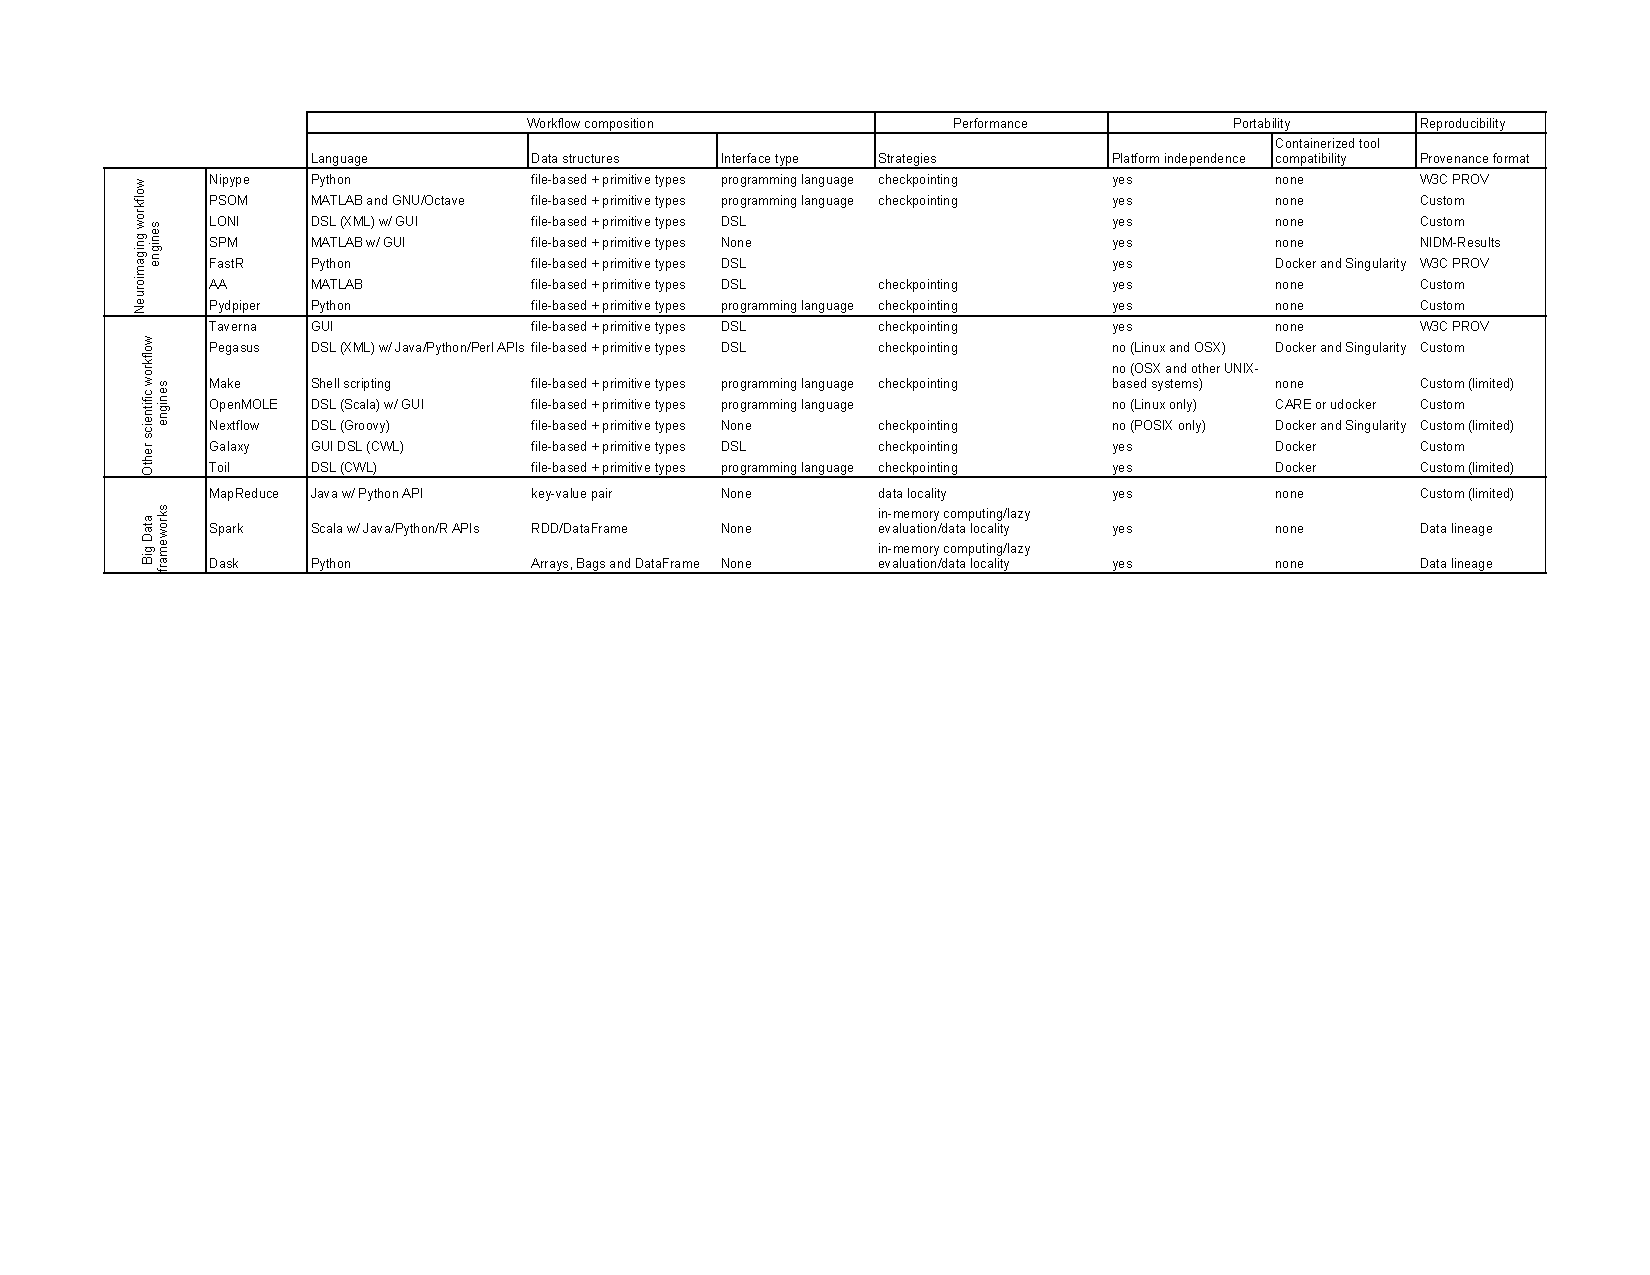
\includegraphics[width=\textwidth,height=\textheight,keepaspectratio]{Figures/summary.pdf}
        \caption{Summary table comparing the 17 workflow engines on four axes:
        workflow composition, performance, portability and reproducibility.}
    \end{sidewaysfigure} 
    \addcontentsline{toc}
        {chapter}{Bibliography} 
        \bibliographystyle{ieeetr}
        \bibliography{bibliography}
\end{document}
